\documentclass[conference]{IEEEtran}

\ifCLASSINFOpdf

\else

\fi


\usepackage{graphicx}
\usepackage{textcomp}
\usepackage{mathtools}

% correct bad hyphenation here
\hyphenation{op-tical net-works semi-conduc-tor}


\begin{document}
 
\title{Competitive co-evolution in robots: \\ heterogeneity vs homogeneity}



\author{\IEEEauthorblockN{Selene Baez Santamaria, Andrea Jemmett, Tommie Kerstens, Enrico Rotundo}
\IEEEauthorblockA{
Vrije Universiteit Amsterdam \\
Amsterdam, Netherlands}}



\maketitle


\begin{abstract}
In the context of robotics, intelligent behaviours are often achieved using neural networks as controllers evolved using  an evolutionary algorithm.
In the case of multiple individuals within a species, controllers can be either homogeneous or heterogeneous.
In this paper, we use competitive co-evolution of homogeneous and heterogeneous controllers in order to investigate its effects on the emergence of specialisation behaviour regarding a herding 

TODO: add what we have discovered!!!!!!!
% TODO: add what we have discovered
\end{abstract}


\IEEEpeerreviewmaketitle


\section{Introduction}
% Evolutionary Algorithms
Evolutionary algorithms (EA) are biology inspired algorithms that, going through multiple steps (e.g., generation, procreation, etc.), are able to evolve entities over time.
Thus, the entities subject to the evolution are referred to as individuals,
%and the EA acts as the digital environment these individuals are born, live, procreate and die in.
and the evolution is usually controlled such that next generations improve along the runs.
In the field of robotics, EAs can be used to evolve the behavioural controller of a robot, these controllers are evolved as individuals in an EA.
% Neural Networks
A Neural Network (NN) is a function estimator that can be used as a controller and its design is natural inspired by the biological nervous system.
In order to employ a NN as a controller, inputs usually come from the sensors making observations of the environment, while the weights are evolved by an EA.
The complete evolutionary process can be run in a simulation which exploits the computer's computational power in order to evaluate many individuals in a reasonable time. 
Robotics employs both EAs and NNs in order to evolve intelligent behaviours that can pursue one or more given goals.

% Solvable tasks
Tasks composition and complexity can vary based on the specific scenario, in general it is subject of many studies aiming to solve different tasks.
For instance, tasks can be relatively small (e.g., moving objects) or more based on collaboration between a number of individuals.
Research investigates collective behaviour in order to asses to which extent collaboration between individuals is feasible.  

% Our task/paper
In this paper, we consider competitive co-evolution within a herding task which consists of a number of shepherds that herd a sheep into a corral.
We evolve NN controllers and assign them to the agents, the latter step can be done with the homogeneous or heterogeneous approach.
While the former employs the same controller instance for each agent, 
%meaning that each shepherd is assigned to the same controller. 
%This one single controller is also the only evolved individual in the EA. 
in the latter each agent gets its own instance of a controller, which is separately evolved by an EA.
% TODO are we going to talk about increasing complexity here?
Moreover, the task complexity can be increased by varying or introducing new agents like adding a fox.

In this paper we employ the aforementioned components within a simulated herding task.
Thus, we recap our objectives in the following list:

\begin{itemize}
	\item To compare homogeneity versus heterogeneity.
	\item To estimate the effect on homo versus heterogeneity of increasingly difficult task.
 	\item To develop controlled experiments through software simulations, using ad hoc libraries.
	\item To collect comprehensive results data.
\end{itemize}
 
\subsection{Research questions}
\label{sec:researchQuestions}
In the herding task, shepherds and sheep have opposing goals.
While the former tries to herd sheep into the corral, the latter tries to escape through the left side of the pasture. 
Thus, species can be competitively co-evolved in a race to evolve strategies to accomplish opposing goals. 
Furthermore, the task complexity can be influenced by varying different parameters such as the number of present agents per each type or their relative movement speeds. 
Another type of dimension used to scale the difficulty is the type of controller used,
Instances of different controller types can be either \textit{static} or \textit{intelligent}.
A \textit{static} controller is simply a predefined set of rules that implements a specific behaviour.
Although an \textit{intelligent} controller is more complex, it is able to  adapt itself over time.
In this paper both the sheep and the shepherds have an \textit{intelligent} controller.
The intelligence of the controller is based on the assumption that since a NN is evolved, the controller has the possibility to adapt to its environment through the evolutionary process. 
This process, in which many strategies are simulated and evaluated, is comparable to a learning process and enables adaptivity. 
Assuming an intelligent sheep we state the following research questions:

\begin{enumerate}
	\item How does the competitive co-evolution affect the relation between homogeneous and heterogeneous shepherds' controllers, in a co-evolved herding task?
	\item How does increasing the number of shepherds increases the need for heterogeneous controllers?
	\item How does increasing task complexity (by adding more sheep) affects the effectiveness of herding?
\end{enumerate}

\subsection{Hypothesis}
\label{sec:hypothesis}
The following hypothesis are in one to one relationship with the aforementioned research questions:

\begin{enumerate}
	\item Shepherds' fitness in the heterogeneous case is overall higher than in the homogeneous case.
	\item The number of shepherds herding one sheep is directly related to their fitness in heterogeneous cases, such that fitness increases as the number of shepherds increases.	
	\item Increasing the number of sheep herd by a fixed number of shepherds decreases the number of corralled sheep.
\end{enumerate}
$H_0$, namely the null hypothesis, is ``Shepherds’ fitness in the heterogeneous case is equivalent to the one of the homogeneous''.
%TODO: add null hyptoesis for H_2 and H_3

\subsection{Contributions}
In this paper we introduce our proposed model for running a herding task in a competitive co-evoulution framework. 
We have built our model and run a thorough set of simulations in order to test the hypothesis detailed in Section~\ref{sec:hypothesis}. 
In what follow, we list the main contributions this paper to the state-of-the-art:
\begin{itemize}
	\item BLA
	\item PIZZA
	\item PASTA
	\item NESPRESSO....what else?
\end{itemize}

This work sheds a tiny light in the topic of competitive co-evoultion by showing to which extent it is feasible in a herding task accomplished by robots.

\subsection{Organization}
%TODO: finish this!
The rest of this paper is organized as follows. 
In Section X, we revise the state-of-the-art related to our research topic. 
In Section Y, we present our model, describing its different components. 
We evaluate the performance of our solution in Section Z. 
Finally, in Section M we draw some conclusions and point out ways to further extend this work.

\section{Literature review}
In this section, we survey the main researches in related work, considering different the following topics: \textit{co-evolution}, \textit{competitive co-evolution}, \textit{evolving NNs} and \textit{homogeneity \& heterogeneity in NNs}.
 
\subsection{Co-evolution}
Co-evolution in its foundation is a natural phenomena.
It describes how the basic principles of evolution are propagated through a dynamic process in which species not only evolve due to the selection pressure produced by an environment, but also due to the selection pressure produced as a by-product of other species evolving within that same environment.
The effects of co-evoultion in butterflies and plants have been studied as early as 1964 in ~\cite{ehrlich1964butterflies}.
Furthermore, the authors of ~\cite{janzen1980coevolution} define co-evolution as ``an evolutionary change in a trait of the individuals in one population in response to a trait of the individuals of a second population''. 
%In 1980 Janzen's \cite{janzen1980coevolution} formalised a clear definition for coevolution:
%`` 'Coevolution' may be usefully defined as an evolutionary change in a trait of the individuals in one population in response to a trait of the individuals of a second population, followed by an evolutionary response by the second populations to the change in the first.''


\subsection{Competitive Co-evolution}
In extension to the broader co-evolution, competitive co-evolution has, as its name suggest, a focus towards competitive elements creating selection pressure.
Dawkins and Krebs describe in~\cite{dawkins1979arms} the dynamics and terminology for competitive coevolution by providing examples of manifestations of competitive coevolution in natural systems. 
The paper captures the pure essential of competitive coevolution giving the following description: ``An adaptation in one lineage (e.g. predators) may change the selection pressure on another lineage (e.g. prey), giving rise to a counter-adaptation. If this occurs reciprocally, an unstable runaway escalation or 'arms race' may result''.

\subsection{Evolving NNs}
The weights of a NN can be evolved when possible configurations of these weights are subjected to selection pressure.
Using this technique, strategies to reach the goals the controlled agent is tempting to achieve become encoded in the ANN.
%get some paper showing simple evolution of NNs
In~\cite{stanley2004competitive}, the authors show that through the complexification of agent controllers in a competitive co-evolutionary setting, the controller's added complexity can be utilized through the generation of more advanced strategies as complexity increases. 
Complexification of the controllers was managed by increasing the size of the ANN gradually during the evolution run.
Resizing the network was achieved using NeuroEvolution of Augmenting Topologies (NEAT).
NEAT allows for the addition of connections and or nodes to a NN while maintaining learned behaviours by keeping the encoded information in the resized NN very close to its previous state.

\subsection{Homogeneity \& Heterogeneity in NNs}
\cite{potter2001heterogeneity} performed a study to a tradeoff of homogeneity versus heterogeneity in the control systems of robots by allowing teams to coevolve their high-level controllers given different levels of difficulty of the task.
The hypothesis was ``simply increasing the difficulty of a task is not enough to induce a team of robots to create specialists''.
Task difficulty was varied by replacing one adversary's passive controller with an active variant supposedly proving that increased difficulty did not justify the use of heterogeneous controllers.
However, increased difficulty was never implemented structurally nor tested methodologically. 

\section{Model design}
%This can be considered as an extension of~\cite{potter2001heterogeneity} because the task, as well as part of the model, are similar. 
In this section we detail our model which aims to simulate a herding task by employing robots with intelligent controllers.
% Herding environment + Task complexity
The herding task involves shepherd robots trying to push sheep robots into a corral, this is further detailed in Section~\ref{sec:herding_task_environment}.
%% Positioning system
%In particular, the positioning system used to control and direct movements of the agents, is described in Section~\ref{sec:positioning_system}. 
% NN_design
Controllers of both shepherds and sheep are modelled as different in an high level manner using NNs.
Thus, their designs are explained in Section~\ref{sec:NN_design} and and how they are evolved is detailed in Section~\ref{sec:controllers_evolution}.
% obstacle_avoidance + NN_output_interpretation
Agents have a simple obstacle avoidance system that allows them to interact with each other, bump into walls and makes the shepherd capable of herding the sheep.
Furthermore, in order to actuate the movements the output from the controller has to be translated into Cartesian coordinates, in order for the simulation engine to move the agents on the screen.    
Both steps are finally specified in Section~\ref{sec:agents_design}.

\subsection{Herding task and environment}
\label{sec:herding_task_environment}
% herding task + environment
The task domain is herding (a sub-domain of the more general pursuit evation task).
Our objective is to simulate shepherd robots trying to push sheep robots into a corral. 
The environment consists of a $l \times l$ squared pasture with fences on the top and bottom.
The corral is positioned on the right side, and the pasture is open on the left side for the sheep to escape.
% Task complexity
We module the task complexity by controlling the number of agents of each type that take part in the task, respectively $D$ for the shepherds (or dogs) and $S$ for the sheep.
Thus, we deploy it as the shepherd to sheep ratio, defined as $\phi = D / S$, where an increased ratio implies a more complex task for the shepherds.

% Positioning system
We use an agent centered polar coordinate system where an agent's position is relative to a second agent of the same type (i.e., shepherd or sheep).
The coordinate system's polar axis passes through the center of the corral and the second agent's position. 
Within this system, a coordinate pair is defined as $\mathbf{p} = (r, b)$, where $r$ is the distance to the second agent (range) and $b$ is the angle from between the two agents, relative to the polar axis (bearing).
In order to define the position of a group of sheep, we take into account the center of mass $\mathbf{gc}$, which is equal to the position of the sheep when there is only one.
% explain how we calculate the gc
The center the sheep group is calculated like the center of mass of a particle system, as following:
$$ \mathbf{gc} = \frac{1}{S} \sum_{i=1}^{S}{\mathbf{x_i}} $$
The overall task environment described here is depicted in Figure~\ref{fig:task_env}. 

\begin{figure}[ht]
	\centering
	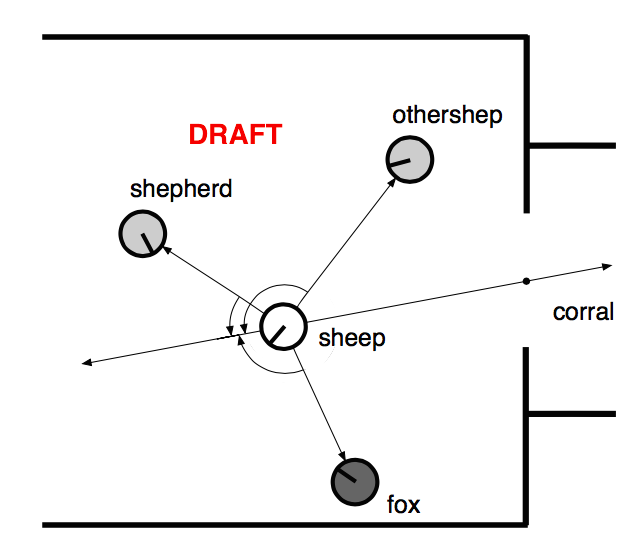
\includegraphics[width=0.8\hsize]{imgs/herding_environment.png}
	\caption{Herding task environment and detail of the positioning coordinates for a group of sheep.}
	\label{fig:task_env}
\end{figure}


\subsection{Neural Networks design}
\label{sec:NN_design}
The controllers for the agents are feedforward neural networks~\cite{bebis1994feed} and each agent contains a multilayer perceptron with one hidden layer.
% Inputs
The inputs for the NNs are a \textit{bias} and one or more instances of \textit{coordinate pairs} (defined in Section~\ref{sec:herding_task_environment}).
While the former is a fixed value, the latter is dynamic and varies depending on the position of the other agents. 
Furthermore, in order to design some NNs able to support scenarios with diverse number of agents, we design two different NNs: the \textit{single-pair} and the \textit{multi-pair} networks. 
% Single-pair NN
With the \textit{single-pair} network, an agent can only see one other agent so the network consists of two input nodes, one for each item of a \textit{coordinate pair} and its hidden layer has three nodes. 
This network is showed in Figure~\ref{fig:single_pair_topology}.
% Multi-pair NN
Alternatively, if the agent can see two other agents it has the \textit{multi-pair} neural network, with four input nodes for the coordinate, and five nodes in its hidden layer. 

Moreover, for every NNs the activation function is a sigmoid function $S(t) = 1 / 1 + \epsilon^{-t}$, centred at $0$. 
The output of the network is a polar \textit{coordinates pair}, namely \textit{target position}, that represents the space point in which the agent will try to move to in the next time step.
Finally, the output of the NN has a range from $(0, 1)$, so in order to convert it into the used positioning system it is  translated into a range of $[0, l]$ for target ratios and $[-\pi, \pi]$ for target bearings. 
 
\begin{figure}[t]
	\centering
	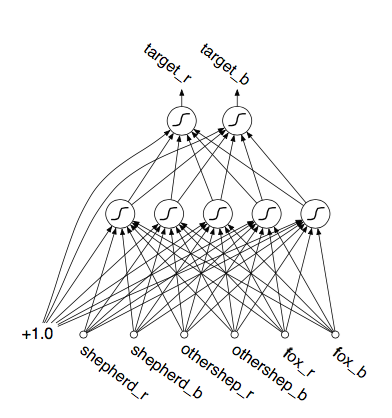
\includegraphics[width=0.8\hsize]{imgs/NN_topology.png}
	\caption{single-pair NN.}
	\label{fig:single_pair_topology}
\end{figure}

\begin{figure}[t]
	\centering
	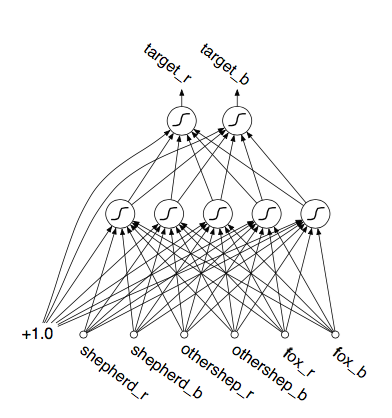
\includegraphics[width=0.8\hsize]{imgs/NN_topology.png}
	\caption{multi-pair NN.}
	\label{fig:multi_pair_topology}
\end{figure}

\vspace{0.5em}
% Shepherds controllers
\subsubsection{Shepherds controllers}
The shepherds evolve \textit{cooperative} behaviours among themselves to successfully herd the sheep.
Therefore, the \textit{competitive} behaviour is against the sheep, who want to escape. 
In order to pursue cooperation, a shepherd needs information about the other shepherds around. 
However, in order to keep the network complexity low we only provide the controller with information for the closest shepherd. 
Similarly, the competition implies a shepherd to have information about the sheep. 
%Following the same motivation, only the closest sheep position is fed into the network. % there's not motivation motivation
Thus, the inputs for a shepherd controller are: 

\begin{enumerate}
	\item \textit{closestSheep\_r}: Distance from this shepherd to the closest sheep.
	\item \textit{closestSheep\_b}: Angle between this shepherd and the closest sheep. 
	\item \textit{closestShepherd\_r}: Distance from this shepherd to the closest shepherd.
	\item \textit{closestShepherd\_b}: Angle between this shepherd and the closest shepherd.
\end{enumerate}

We highlight the third and fourth input are not taken into account in scenarios where there is only one shepherd. 

\vspace{0.5em}
% Sheep controllers
\subsubsection{Sheep controllers}
In case of the sheep, competitive and cooperative collective behaviour is implemented similarly to the sheperd. 
This time, in order to avoid the shepherd and be able to escape, sheep have information about the closest shepherd. 
Yet, they have a strong preference to stay in a group and so need information about the closest sheep around them in order to pursue this goal. 
Thus, the inputs for a sheep's controller are:

\begin{enumerate}
	\item \textit{closestShepherd\_r}: Distance from this sheep to the closest shepherd.
	\item \textit{closestShepherd\_b}: Angle between this sheep and the closest shepherd.
	\item \textit{closestSheep\_r}: Distance from this sheep to the closest sheep.
	\item \textit{closestSheep\_b}: Angle between this sheep and the closest sheep.
\end{enumerate}

Once again, we point out the third and fourth inputs are not taken into account in scenarios where there is only one sheep. 

\subsection{Evolution of controllers}
\label{sec:controllers_evolution}
The algorithm used to evolve the controllers follows the frameworks of evolutionary strategies. 
The genome is an array of doubles consisting of the weights for the neural network: 17 for the \textit{simple-pair} network and 37 for the \textit{multi-pair} network. 
We use the ($\mu + \lambda$) strategy, with $\mu = 10$ and $\lambda = 100$~\cite{eiben2003introduction}. 
Furthermore, each individual in a population is evaluated with the best individuals from the other populations, following an elitist approach.
Different fitness functions are created for each type of agent, we Hereby explain each of them and their motivation.

\vspace{0.5em}
\subsubsection{Shepherd fitness function}
In order to show the shepherd fitness function, we introduce here~\eqref{eq:gcDist}, the euclidean distance from the sheep center of group mass $gc$ (see Section~\ref{sec:herding_task_environment}) to the corral position $cr$.
Given $t$ as incremental index of the simulation time steps, it is defined as:
% GROUP CENTER OF MASS DISTANCE
\begin{equation} \label{eq:gcDist}
gcd(t) = \sqrt{(cr_x - gc_x(t))^2 + (cr_y - gc_y(t))^2}
\end{equation}
This metric grows as the group of sheep distance itself from the corral in the attempt of escaping.
Furthermore, at every time step a \textit{bonus} is awarded for corralling a sheep or a \textit{penalty} is deducted for letting a sheep escape, after which the sheep is eliminated from further computations. 
Each of these stimulus is regulated by the time within the simulation, meaning that a bonus/penalty is larger the earlier it happens. 
% SHEPHERD BONUS
\begin{equation} \label{eq:bonus}
bonus(t) = - stimulusMultiplier * (T - t)
\end{equation}
% SHEPHERD PENALTY
\begin{equation} \label{eq:penalty}
penalty(t) = stimulusMultiplier * (T - t)
\end{equation}
Where $T$ is the number of total steps (1500 in our experiments) and $t$ is the number of elapsed steps when the simulation stopped.
Note that $stimulusMultiplier$ is a fixed coefficient used to control weight of the aforementioned values. 
Finally, the fitness for shepherds is defined as the cumulative distance from the sheep center to the corral position~\eqref{eq:gcDist} taking into account bonuses~\eqref{eq:bonus} and penalties~\eqref{eq:penalty}, over every simulation time step:
% SHEPHERD FITNESS
\begin{equation} \label{eq:shep_fitness}
f_{sheph} = \sum_{i=1}^{1500} gcd(i)	+ bonus(i) + penalty(i)
\end{equation}
In order to to observe a herding behaviour,~\eqref{eq:shep_fitness} has to be minimized.
Note that the fitness is the same among a group of shepherds, since all the components reflect on the group's performance. 
This design choice is motivated by the fact that shepherds must work together to achieve a common goal. 

\vspace{0.5em}
\subsubsection{Sheep fitness function}
The fitness for a sheep is determined by its own distance to the corral. 
% SHEEP DISTANCE
\begin{equation} \label{eq:sheep_dist}
sd(t) = \sqrt{(cr_x - sheep_x(t))^2 + (cr_y - sheep_y(t))^2}
\end{equation}
In scenarios where there is more than one sheep, a group component is added to motivate sheep to stay in groups. 
This is the ratio $\phi$ of the group calculated as the distance from the furthest sheep $\alpha$ to the center of mass $gc$ in a specific time step. 
% SHEEP RATIO
\begin{equation} \label{eq:sheep_ratio}
\phi(t) = \sqrt{(\alpha_x(t) - gc_x(t))^2 + (\alpha_y - gc_y(t))^2}
\end{equation}
Similarly to the shepherds, bonuses and penalties are given when a sheep escapes or is corralled, accordingly:
% SHEEP BONUS
\begin{equation} \label{eq:sheep_bonus}
f_{sheep}(x) = f_{sheep}(x) + stimulusMultiplier * (T - t)
\end{equation}
% SHEEP PENALTY
\begin{equation} \label{eq:sheep_pen}
f_{sheep}(x) = f_{sheep}(x) - stimulusMultiplier * (T - t)
\end{equation}
Where $T$ is the number of total steps (1500 in our experiments) and $t$ is the number of elapsed steps when the simulation stopped.
Since larger distances but smaller ratios are desired, the fitness function is determined as the individual distance minus the group ratio, added over the simulation time steps. 
% SHEEP FITNESS
\begin{equation} \label{eq:sheep_fitness}
f_{sheep}(x) = \sum_{i=1}^{1500}(sd(i) - 0.8 * \phi(i))
\end{equation}


\subsection{Agents}
\label{sec:agents_design}
% Obstacle avoidance
Given the output of the networks, the agents will try to move into a position.
However, both types of agents have obstacle avoidance built into their behaviour which might prevent them from moving to the target position. 
% Interpreting the Neural Network output
Since the output for the network is represented as polar coordinates centered at the sheep center of mass, they are translated into Cartesian coordinates in the pasture. 
%TODO: Others properites: like speed....




\section{Experimental results}
\label{sec:experiment}
In order to answer the research questions listed in {Section~\ref{sec:researchQuestions}} and test its corresponding hypothesis in {Section~\ref{sec:hypothesis}}, we perform co-evolution across 100 generations. 
We run the simulation 40 times and perform statistical analysis to get 95\% confidence intervals.

\subsection{Implementation}
%TODO: the implementation is the description of the instance of our model used to run the experiments, this means that all parameters should be defined (name+meaning) in the model section and instanciated in the implementation.  The impl. is not much about the code/classes etc unless we came up with a novel algortihm....
The project is coded in Java with use of \textit{Mason} for handling agents and their movements. In order to introduce evolutionary computing, we combine it with \textit{ECJ}. We use \textit{neuroph} as the library for neural networks. 
\textbf{TODO: Since ECJ can only do maximization problems, the shepherd fitness is taken as 
fitness = - cummulative distance}
\textbf{TODO: Mention value for parameters, for example stimulusMultiplier = pasture width, groupMultiplier = 0.8}
A simulation consists of 2.5 second divided in 1500 discrete time steps. At every time step, an agent propagates the inputs through its neural network and computes a target position.
\textbf{TODO: pseudocode? diagram?}




\subsubsection{Environment}
pasture=37x37 foot, $l = 37$ foot


\subsubsection{Neural Networks}
TODO

\subsubsection{Evolution}
In order to calculate the fitness for an individual, all controllers are evaluated through 10 trials of the task and the average is taken as fitness.
Every trial runs for a maximum of 2.5 seconds. 
In cases where there is more than one sheep, a complex network is assigned to all sheep. 
The simulation ends before the time elapses if all but one sheep escape or get corralled. 
The reason for leaving one sheep left in the pasture when ending the simulation is that the number of inputs for the sheep controllers is fixed before the beginning of a trial, and having no other sheep left would lead to null inputs and misbehaviour. 
In cases where there is only one sheep, a simple controller is assigned. 
Thus, the sheep must either be corralled or has to escape in order for the simulation to stop before the time expires.

In homogeneous set-ups we evolve one controller per type of agent, meaning we have two subpopulations, one for shepherds and one for sheep, coevolving. 
However, to create heterogeneity a population per agent is created. 
For example, in a scenario with two shepherds and one sheep, there is a total of three subpopulations, two of them cooperating among each other and competing with the third one.  

\subsubsection{Agents properties and functioning}
Shepherds avoid bumping into fences, the corral or other agents within a 3 simulation distance units. 
Meanwhile, the sheep can only avoid fences and other agents within a 2 simulation distance units.



\subsection{Performance details}
\label{sec:experiments_performances}
% Homo vs Etero experiment
\vspace{0.5em}
\subsubsection{Controllers comparison}
We first consider experiments that relate to $H_1$. To investigate the difference between homogeneous and heterogeneous controllers for the shepherd agents, we explore scenarios with fixed number of agents. 
\begin{itemize}
	\item 2 homogeneous shepherds vs 1 sheep
	\item 2 heterogeneous shepherds vs 1 sheep
	\item 3 homogeneous shepherds vs 1 sheep
	\item 3 heterogeneous shepherds vs 1 sheep
\end{itemize}

% Need for heterogeneous controllers
\vspace{0.5em}
\subsubsection{Need for heterogeneousity: shepherds number}
In order to test $H_2$, we compare different scenarios with different number of shepherds corralling one sheep:
\begin{itemize}
	\item 1 shepherd vs 1 sheep	
	\item 2 homogeneous shepherds vs 1 sheep
	\item 3 homogeneous shepherds vs 1 sheep
	\item 2 heterogeneous shepherds vs 1 sheep
	\item 3 heterogeneous shepherds vs 1 sheep
	
\end{itemize}

% Task complexity: more sheep!
\vspace{0.5em}
\subsubsection{Task complexity: sheep number}
Finally, $H_3$ is approached by comparing scenarios with a fixed number of shepherds, in this case three, and different number of sheep. 
\begin{itemize}
	\item 3 heterogeneous shepherds vs 1 sheep
	\item 3 heterogeneous shepherds vs 2 homogeneous sheep
	\item 3 heterogeneous shepherds vs 3 homogeneous sheep
\end{itemize}
The second and third round of experiments regulate the task complexity by having different sheep to shepherd ratios. 
\begin{itemize}
	\item one shepherd one sheep = 1 ratio
	\item two shepherds one sheep = 0.5 ratio
	\item three shepherds one sheep = 0.33 ratio
	
	\item three shepherd one sheep = 0.33 ratio
	\item three shepherd two sheep = 0.66 ratio
	\item three shepherd three sheep = 1
\end{itemize}


\section{Results}
In this section we present the results of the experiment detailed in Section ~\ref{sec:experiment}.

\vspace{0.5em}
\subsubsection{Homogeneous vs heterogeneous}
\begin{figure}[ht]
	\centering
	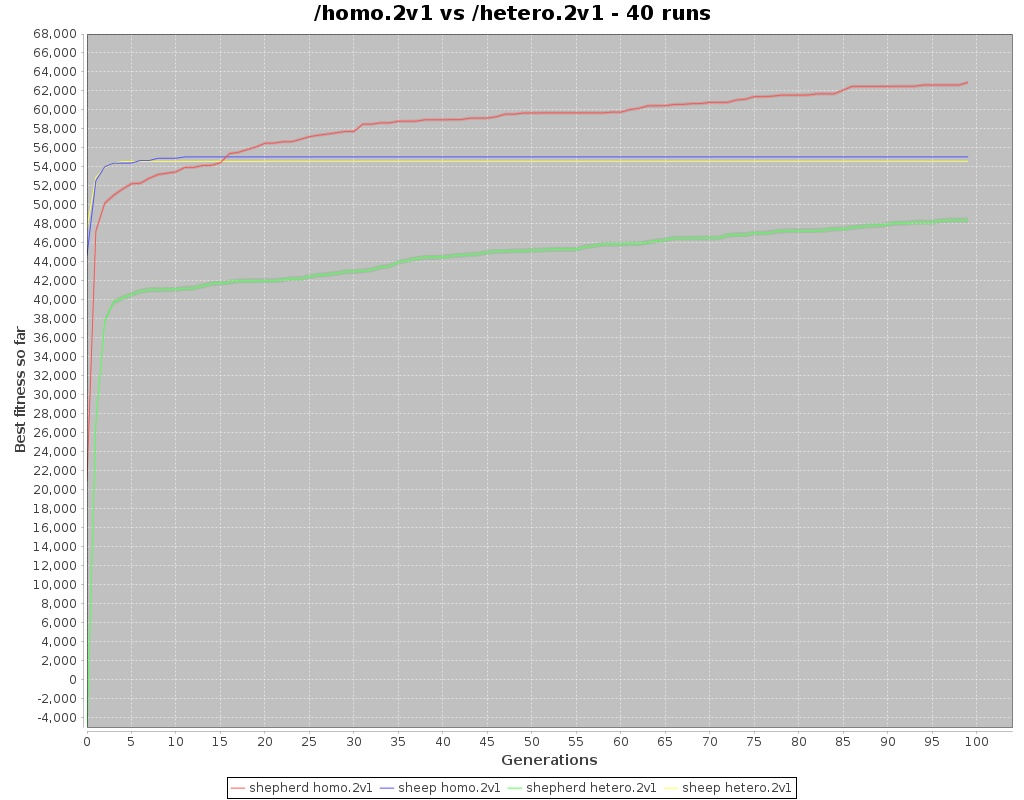
\includegraphics[width=3.3in]{imgs/homo2v1-hetero2v1-bestSoFar.jpeg}
	\caption{Best individuals fitness in scenario with two shepherds and one sheep. Both homogeneous and heterogeneous settings are shown}
	\label{fig:2v1_homo_vs_hetero}
\end{figure}

\begin{figure}[ht]
	\centering
	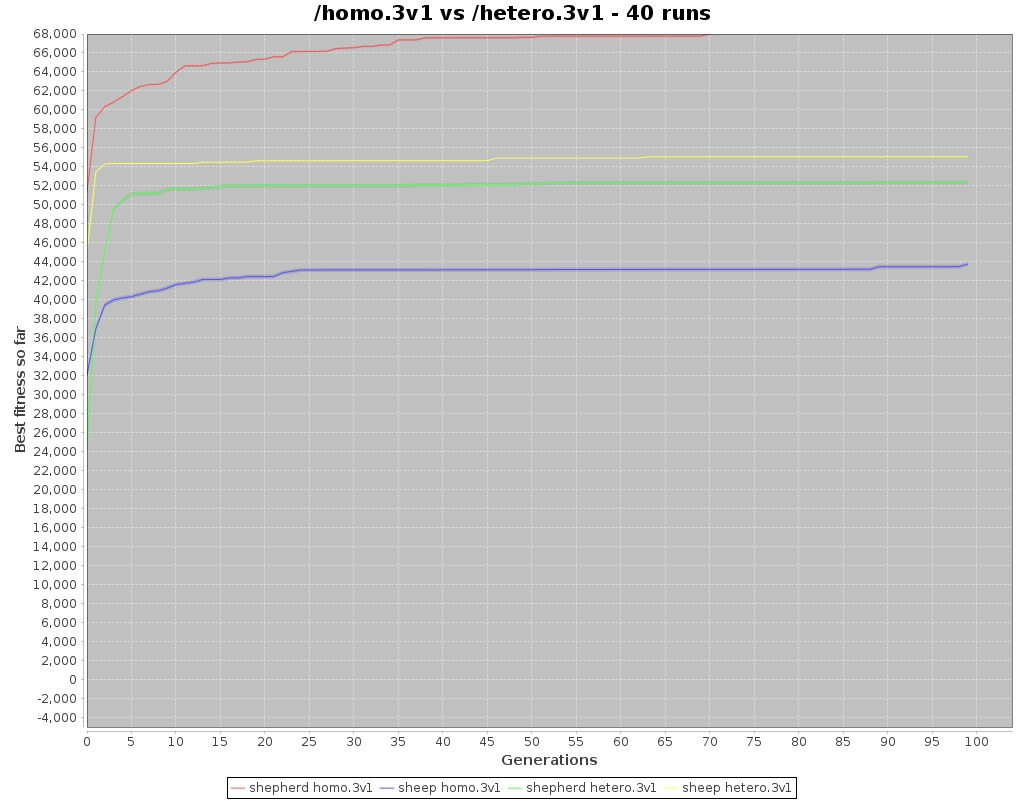
\includegraphics[width=3.3in]{imgs/homo3v1-hetero3v1-bestSoFar.jpeg}
	\caption{Best individuals fitness in scenario with three shepherds and one sheep. Both homogeneous and heterogeneous settings are shown}
	\label{fig:3v1_homo_vs_hetero}
\end{figure}

\textbf{TODO: interpret graph. Shepherd do better in homo. Sheep does better with hetero dogs}

\vspace{0.5em}
\subsubsection{Adding more shepherds}

\begin{figure}[ht]
	\centering
	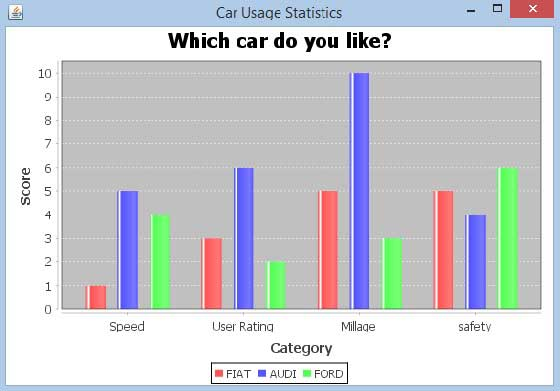
\includegraphics[width=3.3in]{imgs/barchart.jpg}
	\caption{Bar chart for corralled cases in heterogeneous setting. Shows mean, best and worse for scenarios with one, two and three shepherds herding one sheep}
	\label{fig:corralled_oneSheep}
\end{figure}

\begin{figure}[ht]
	\centering
	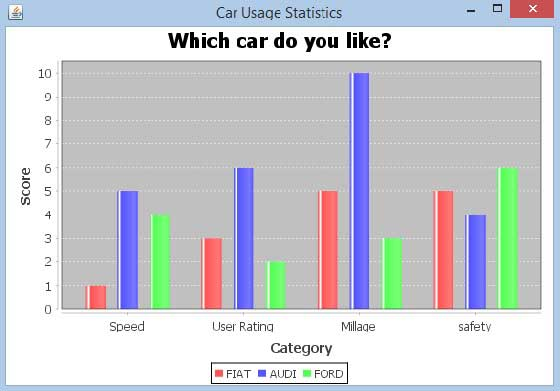
\includegraphics[width=3.3in]{imgs/barchart.jpg}
	\caption{Bar chart for escaped cases in heterogeneous setting. Shows mean, best and worse for scenarios with one, two and three shepherds herding one sheep}
	\label{fig:escaped_oneSheep}
\end{figure}

\textbf{TODO: Interpret trend as more shepherd get involved, how does hetero does?}
\textbf{TODO: consider including same graphs in homogeneous scenarios}

\vspace{0.5em}
\subsubsection{Adding more sheep}
o	Look at percentage of corralled and escaped of last generation


\begin{figure}[ht]
	\centering
	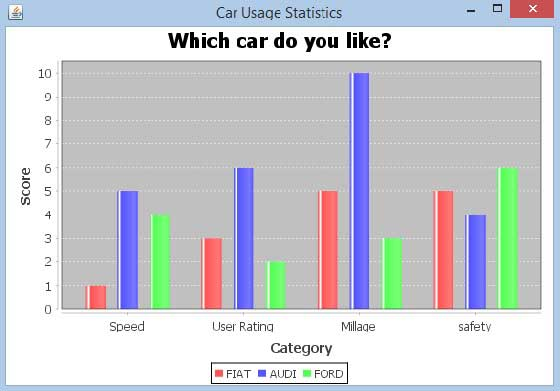
\includegraphics[width=3.3in]{imgs/barchart.jpg}
	\caption{Bar chart for corralled cases in heterogeneous setting. Shows mean, best and worse for scenarios with three shepherds herding one, two and three sheep}
	\label{fig:corralled_threeShepherd}
\end{figure}

\begin{figure}[ht]
	\centering
	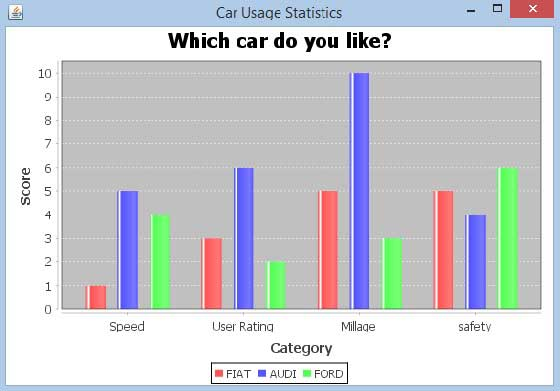
\includegraphics[width=3.3in]{imgs/barchart.jpg}
	\caption{Bar chart for escaped cases in heterogeneous setting. Shows mean, best and worse for scenarios with three shepherds herding one, two and three sheep}
	\label{fig:escaped_threeShepherd}
\end{figure}

\textbf{TODO: Interpret trend as more sheep need to be corralled (task is more complex)}


\section{Conclusion}
The conclusion goes here.

%\subsection{Future work}
%TODO: future work



\bibliographystyle{abbrv}
\bibliography{bibliography}



\end{document}

